%%%%%%%%%%%%%%%%%%%%%%%%%%%%%%%%%%%%%%%%%%%%%%%%%%%%%%%%%%%%%%%%
%% Author: Anshuman Dhuliya (144050002)
%% Document: CV
%% Title: Anshuman Dhuliya CV
%% Commands:
%%     make             # produces the main.pdf file
%%     make clean       # cleans the temporary files
%%     make tar         # makes the tgz file containing all necessary contents
%%     make show        # shows the pdf on evince
%% use: `convert a.jpg eps2:a.eps`  %% to insert jpeg images as eps
%% use: `identify a.eps` command to find the dimensions of a.eps
%%%%%%%%%%%%%%%%%%%%%%%%%%%%%%%%%%%%%%%%%%%%%%%%%%%%%%%%%%%%%%%%

\documentclass[a4paper,12pt]{article}

\newcommand{\Space}{\hspace{1ex}}
\newcommand{\Sp}{\hspace{1ex}}
\newcommand{\Heading}[1]{\textbf{\itshape\normalsize #1}}

\usepackage[a4paper,lmargin=1.2cm,rmargin=1.2cm,tmargin=1.5cm,bmargin=1.5cm]{geometry}
\usepackage{tabu}

\usepackage{array}
\newcolumntype{M}[1]{>{\centering\arraybackslash}m{#1}}
\newcolumntype{R}[1]{>{\raggedleft\arraybackslash}m{#1}}

\usepackage{fancyhdr}
\pagestyle{fancy}
\rfoot{\textit{If you can read this, thank a Teacher! -- Anonymous}\Sp{}\Sp{}\Sp{}\Sp{}\Sp{}\Sp{}\textbf{\LaTeX}}
\renewcommand{\headrulewidth}{0pt}

\setlength\tabcolsep{0pt}

\usepackage{graphicx}

\begin{document}
\begin{flushleft}

\pagenumbering{gobble} % no page numbers


%    \begin{tabular}{|l{0.75\textwidth}|l{0.25\textwidth}|}
    \begin{tabular*}{\textwidth}{m{0.85\textwidth} m{0.15\textwidth} }
        {\LARGE{}\rule[3ex]{0ex}{0ex}\textbf{Anshuman Dhuliya}}\newline%
        {\rule[3ex]{0ex}{0ex}\large{}\itshape{}Research Scholar, CSE Department, IIT Bombay} \newline%
        {\rule[3ex]{0ex}{0ex}\large{}\itshape{}Senior Research Associate, AJIT Project, EE Department, IIT Bombay} \newline%
        \rule[3ex]{0ex}{0ex}{Flat 120, 2$^{\textit{nd}}$ Floor, Type-2B Bldg 20, Hill Side, Next to Manas\newline%
IIT Bombay Campus, Mumbai, Maharashtra, 400076\newline%
        Mob: +91 90045 21241, anshumandhuliya@gmail.com, dhuliya@cse.iitb.ac.in}

&  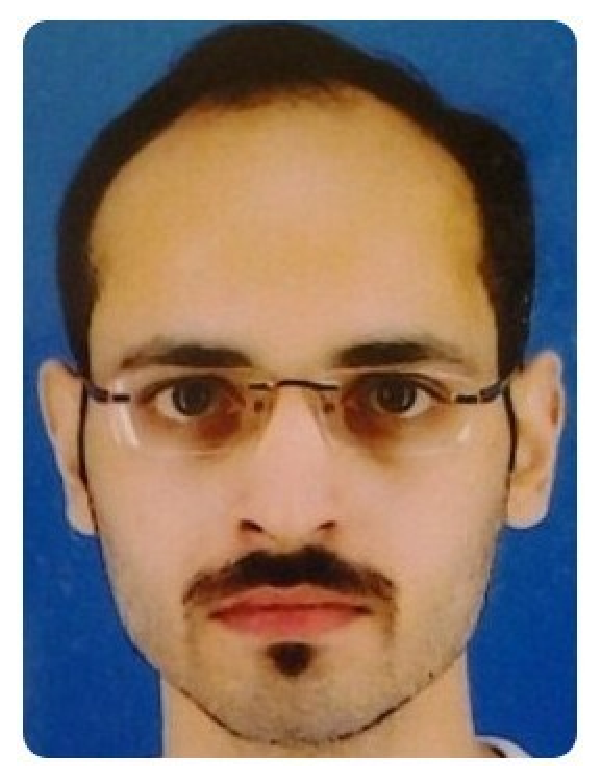
\includegraphics[natwidth=273,natheight=360,width=0.15\textwidth]{images/anshuman1.eps} \\
\end{tabular*}
\rule[1pt]{\textwidth}{2pt}
\begin{tabular*}{\textwidth}{m{0.95\textwidth} m{0.05\textwidth} }
{\itshape{}\rule[3ex]{0ex}{0ex}I am passionate about
computer technology with special interests in
compilers, interpreters and computer processors.
I am enthusiastic about managed and unmanaged cloud machines.

% Let $P$ be the set of people fond
%   of program analysis and compiler techonology.
%   Let $W$ be the set of people who are passionate about their work
%   and share their knowledge.
%   I am $\in P \cap W$.\newline%
} & \\
\end{tabular*}

    \vspace{3mm}
\begin{tabular}{ m{0.75\textwidth}| R{0.25\textwidth}}
\multicolumn{2}{l}{\Heading{Experience}} \\
    \hline
    \hline
    \rule[3ex]{0ex}{0ex}Senior Research Associate, AJIT Processor, \textit{IIT Bombay} \newline{}India's First Indigenous General Purpose CPU & Jun 2017 - Present\\ \hline

    \rule[3ex]{0ex}{0ex}Research Scholar, CSE Department, \textit{IIT Bombay} \newline{}Program Analysis and Compilers & Jun 2014 - Present\\ \hline

    \rule[3ex]{0ex}{0ex}Head Teaching Assistant, \textit{IIT GOA} \newline{}Introduction to Computer Programming Course with C++ (CS101) & Aug 2016 - Dec 2016\\ \hline

    \rule[3ex]{0ex}{0ex}Invited Speaker, \textit{Sardar Patel Institute of Technology, Mumbai} \newline{}Prolog based Expert Systems & 2016\\ \hline

    \rule[3ex]{0ex}{0ex}Invited Speaker, \textit{RAIT, Navi Mumbai} \newline{}Artificial Intelligence & 2016\\ \hline

    \rule[3ex]{0ex}{0ex}Head Teaching Assistant, \textit{Indian Institute of Technology Bombay} \newline{}Introduction to Computer Programming Course with C++ (CS101) & Jul 2015 - Dec 2016\\ \hline

    \rule[3ex]{0ex}{0ex}Adhoc Faculty, \textit{RGUKT, Kadapa, AP (AP Government Initiative)} \newline{}Compilers, Computer Architecture& Jul 2013 - Jul 2014\\ \hline

    \rule[3ex]{0ex}{0ex}Freelancer Trainer, \textit{Initiated education startup codewalker.in} \newline{}Java, J2EE, C++, Python, Linux& Nov 2009 - Jun 2011\\ \hline 

    \rule[3ex]{0ex}{0ex}Lecturer, \textit{Galgotia's College of Engineering and Technology (GCET)} \newline{}Java, Web Technologies& Apr 2009 - Sep 2009\\ \hline 

    \rule[3ex]{0ex}{0ex}J2EE Application Maintainer, \textit{Nucleus Software Exports Limited (NSEL)} \newline{}Java, J2EE, OracleDB& Sep 2008 - Feb 2009\\ \hline 
\end{tabular}

\vspace{3mm}
\begin{tabular}{ m{0.2\textwidth} | m{0.45\textwidth} | M{0.1\textwidth} |M{0.1\textwidth} |M{0.15\textwidth}}
\multicolumn{5}{l}{\Heading{Education}} \\
    \hline
    \hline
    \multicolumn{1}{>{\centering\arraybackslash}m{0.2\textwidth}}{\textbf{\rule[13pt]{0ex}{0ex}}} & \multicolumn{1}{>{\centering\arraybackslash}m{0.35\textwidth}}{\textbf{Institute}} & \multicolumn{1}{>{\centering\arraybackslash}m{0.1\textwidth}}{\textbf{From}} & \multicolumn{1}{>{\centering\arraybackslash}m{0.1\textwidth}}{\textbf{To}} & \multicolumn{1}{>{\centering\arraybackslash}m{0.15\textwidth}}{\textbf{Marks}} \\ \hline

    \rule[13pt]{0ex}{0ex}Ph.D (Computers) & \Space{}IIT Bombay & 2014 & Present & 9.60 CGPI\\ \hline
    \rule[13pt]{0ex}{0ex}M.Tech (IT) & \Space{}IIIT Allahabad & 2011 & 2013 & 9.55 CGPI\\ \hline
    \rule[13pt]{0ex}{0ex}B.Tech (CSE) & \Space{}Galgotia's GCET, Noida& 2004 & 2008 & 67.72\%\\ \hline
    \rule[13pt]{0ex}{0ex}12$^{th}$ & \Space{}ISC & 2002 & 2003 & 79.50\%\\ \hline
    \rule[13pt]{0ex}{0ex}10$^{th}$ & \Space{}ICSE & 2000 & 2001 & 86.00\%\\ \hline
\end{tabular}

    \vspace{3mm}
\begin{tabular}{ m{0.95\textwidth} M{0.05\textwidth}}
\multicolumn{2}{l}{\Heading{Publications \& Discourse}} \\
    \hline
    \hline
\rule[13pt]{0ex}{0ex}\texttt{Dhuliya, A. and Komondoor, R., and Khedker, U., 2019, July 12-13. Demand Driven Program Analysis with Synergistic Program Analyzer (SPAN), Software Engineering Research in India Update Meeting (SERI 2019)} & \\ \hline

\rule[13pt]{0ex}{0ex}\texttt{Dhuliya, A. and Komondoor, R., and Khedker, U., 2020, July 9-11. Program Analysis with Synergistic Program Analyzer (SPAN), Software Engineering Research in India Update Meeting (SERI 2019)} & \\ \hline

\rule[13pt]{0ex}{0ex}\texttt{Wrote about me: Sai Anirudh Karre, Lalit Mohan, Y. Raghu Raghu Reddy, K.V. Raghavan, R.D. Naik, Rahul Purandare, and Amey Karkare. 2019. A report on 1st Software Engineering Research in India Update Meeting (SERI 2019). SIGSOFT Softw. Eng. Notes 44, 3 (July 2019), 41–42. DOI:https://doi.org/10.1145/3356773.3356805} & \\ \hline

\rule[13pt]{0ex}{0ex}\texttt{Dhuliya, A. and Tiwary, U.S., 2013, November. An associative classifier based on the concept of analogy and human learning. In Multimedia, Signal Processing and Communication Technologies (IMPACT), 2013 International Conference on (pp. 297-301). IEEE} & \\ \hline
\end{tabular}

%\begin{tabular}{| m{0.3\textwidth} | m{0.3\textwidth} | m{0.3\textwidth} |}
%\hline
%Anshuman Dhuliya &  my photo &  my photo \\ \hline
%\end{tabular}
%
%\begin{tabular}{| m{5cm} | m{3cm} | m{3cm} | m{3cm} | m{3cm} |}
%\hline
%Anshuman &  my photo &  my photo &  my photo &  my photo \\ \hline
%\end{tabular}
%
%\begin{tabular}{| m{2cm} | m{3cm} | m{3cm} | m{3cm} | m{3cm} | m{3cm} |}
%\hline
%Anshuman &  my photo &  my photo &  my photo &  my photo &  my photo \\ \hline
%\end{tabular}
%    \vspace*{\fill}
%
%
%
%\begin{tabu} to \textwidth { | X[l] | X[c] | X[r] | }
% \hline
% item 11 & item 12 & item 13 \\
% \hline
% item 21  & item 22  & item 23  \\
%\hline
%\end{tabu}

%\vspace*{\fill}
%\rule[1pt]{\textwidth}{2pt}
%\newpage

\vspace{1em}
\begin{tabular}{ m{0.1\textwidth} m{0.9\textwidth}}
\multicolumn{2}{l}{\Heading{Projects \& Achievements}} \\
    \hline
    \hline
\rule[13pt]{0ex}{0ex}(2020) & Developed custom backend in LLVM compiler infrastructure
for AJIT general purpose processor, IIT Bombay. AJIT is India's first indigenous general purpose processor. \\
\rule[13pt]{0ex}{0ex}(2020) & Built (and still maintaining) a stable buildroot toolchain
for AJIT processor, IIT Bombay. \\
\rule[13pt]{0ex}{0ex}(2020) & Developed SPAN Demand Driven Program Analysis Framework in Python/Cython. \\
\rule[13pt]{0ex}{0ex}(2019) & Developed Sparc Assembly Instruction ReOrdering (SPAIRO)
to improve performance of AJIT processor, IIT Bombay. \\
\rule[13pt]{0ex}{0ex}(2019) & Designed and delivered two day ACM Summer School Workshop on Clang/LLVM internals.\\
\rule[13pt]{0ex}{0ex}(2018) & Developed SLANG Clang/LLVM Checker to convert Clang AST to SPAN IR (towards PhD Thesis). \\
\rule[13pt]{0ex}{0ex}(2017) & Developed SPAN Program Analysis Framework in Python/Cython (towards PhD Thesis). \\
\rule[13pt]{0ex}{0ex}(2015) & Implemented RAFT using GoLang (a distributed consensus algorithm), IIT Bombay. \\
\rule[13pt]{0ex}{0ex}(2014) & Implemented standard IPv4 stack on 8051 processor with 128 byte RAM and 4KiB ROM, IIT Bombay. \\
\rule[13pt]{0ex}{0ex}(2013) & Developed RIMINET (a novel cognitive architecture) towards M.Tech thesis. \\
\rule[13pt]{0ex}{0ex}(2012) & Cleared Round 1 of Google Code Challenge. \\
\rule[13pt]{0ex}{0ex}(2011) & Top 1\% Gate 2011 Ranker. \\
\rule[13pt]{0ex}{0ex}(2009) & Best New Joinee J2EE Developer Award at Nucleus Software. \\
\rule[13pt]{0ex}{0ex}(2009) & Developed Faculty Leave Management System using J2EE for Galgotia's College.\\
\rule[13pt]{0ex}{0ex}(2009) & Sun/Oracle Certified Java Programmer. \\
\end{tabular}

    \vspace{3mm}
\begin{tabular}{ m{0.45\textwidth}  M{0.05\textwidth} |m{0.45\textwidth} M{0.05\textwidth}}
    \multicolumn{4}{l}{\Heading{Skills \& Hobbies}} \\
    \hline
    \hline
    %\multicolumn{1}{>{\centering\arraybackslash}m{0.2\textwidth}}{\textbf{\rule[13pt]{0ex}{0ex}}}
    \multicolumn{2}{>{\centering\arraybackslash}m{0.35\textwidth}}{\textbf{Skills}}
    & \multicolumn{2}{>{\centering\arraybackslash}m{0.15\textwidth}}{\textbf{Hobbies}}
    \\ \hline

    \rule[13pt]{0ex}{0ex}Design and Implement Program Analyses & &
    \Sp{}Travelling \& Long Drives & \\ \hline
    \rule[13pt]{0ex}{0ex}LLVM Compiler Backend Development & &
    \Sp{}Working on Cognitive Architectures & \\ \hline
    \rule[13pt]{0ex}{0ex}Clang/LLVM Checker Development & &
    \Sp{}Wildlife Photography  & \\ \hline
    \rule[13pt]{0ex}{0ex}C/C++/Python Based Development & &
    \Sp{}Hobby Projects Development & \\ \hline
    \rule[13pt]{0ex}{0ex}Cloud Application Development (Google, DO)& &
    \Sp{}Playing Violin and Sketching & \\ \hline
    % \rule[13pt]{0ex}{0ex}Clang Checker Development & \\ \hline
\end{tabular}

\vspace*{\fill}
\rule[1pt]{\textwidth}{2pt}

\vspace{3mm}
\begin{tabular}{ m{0.95\textwidth} M{0.05\textwidth}}
    \multicolumn{2}{l}{\Heading{References}} \\
    \hline
    \hline
    \rule[13pt]{0ex}{0ex}\texttt{Prof. Uday Khedker, Ex-Head Computer Science Department, IIT Bombay. (uday@cse.iitb.ac.in)} & \\ \hline

    \rule[13pt]{0ex}{0ex}\texttt{Prof. Raghavan Komondoor, Department of Computer Science and Automation, IISc Bangalore. (raghavan@iisc.ac.in)} & \\ \hline

    \rule[13pt]{0ex}{0ex}\texttt{Prof. Madhav P. Desai, Electrical Engineering Department, IIT Bombay. (madhav@ee.iitb.ac.in)} & \\ \hline

    \rule[13pt]{0ex}{0ex}\texttt{Prof. Amitabha Sanyal, Ex-Head Computer Science Department, IIT Bombay. (as@cse.iitb.ac.in)} & \\ \hline

    \rule[13pt]{0ex}{0ex}\texttt{Prof. Supratim Biswas, Computer Science Department, IIT Bombay. (sb@cse.iitb.ac.in)} & \\ \hline

    \rule[13pt]{0ex}{0ex}\texttt{Prof. Uma Shanker Tiwari, Intelligent Systems Department,
    Indian Institute of Information Technology - Allahabad (ust@iiita.ac.in)} & \\ \hline

\end{tabular}

\vspace{2em}
I declare that all the information presented above is correct
to the best of my knowledge.

\vspace{2em}

Best.

\vspace{2em}
Anshuman Dhuliya


\vspace*{\fill}
\rule[1pt]{\textwidth}{2pt}

\end{flushleft}
\end{document}


